\begin{frame}
 \frametitle{Plane from Point and two Directions}

\begin{columns}
  \column{6cm}
  Point $P_0$, with position vector $\textbf{r}_0$;\\
  Non-parallel directions $\textbf{u}$ and $\textbf{v}$.
  \column{6cm}
    $\mathcal{P}$: plane through $P_0$ and \\
    parallel to both $\textbf{u}$ and $\textbf{v}$.
\end{columns}

\begin{columns}
  \column{5.5cm}
  \only<2>{Normal direction $\textbf{n} = \textbf{u} \times \textbf{v} \neq \textbf{0}$ \\
  \medskip \textcolor[rgb]{0.98,0.00,0.00}{Implicit vectorial equation}:
  $$P(\textbf{r}) \text{ is on } \mathcal{P} \Longleftrightarrow \boxed{(\textbf{r}-\textbf{r}_0) \cdot \textbf{n} = 0}$$
  Interpretation:\\
  $$\text{Vol}(R(\textbf{r} - \textbf{r}_0,\textbf{u},\textbf{v})) = 0$$}
  \only<3>{$P(\textbf{r})$ is on the plane $\mathcal{P}$ $\leftrightarrow$\\
  \medskip
    $\textbf{P}_0\textbf{P}$ is a combination of $\textbf{u}$, $\textbf{v}$
    $\leftrightarrow$\\
    \medskip
    There are scalars $s$, $t$ such that \\
    $\textbf{r}-\textbf{r}_0= s\textbf{u} + t\textbf{v} \leftrightarrow $\\
    \medskip
    \textcolor[rgb]{0.98,0.00,0.00}{Parametric vectorial equation}:
    $$\boxed{ \textbf{r} = \textbf{r}_0 + s\textbf{u} + t\textbf{v} \; }$$
    for some parameters $s$ and $t$}
  \only<4>{
  \textcolor[rgb]{0.98,0.00,0.00}{Parametric vectorial equation}:
  $$\textbf{r} = \textbf{r}_0 + s\textbf{u} + t\textbf{v}$$
  $P_0(x_0,y_0,z_0)$, $P(x,y,z)$\\
  $\textbf{u} = \langle u_1,u_2,u_3\rangle$,
  $\textbf{v}=\langle v_1,v_2,v_3\rangle$\\
  \medskip\textcolor[rgb]{0.98,0.00,0.00}{Parametric scalar equations}:
  $$\left\{ \begin{array}{ll}
           x = & x_0 + su_1+tv_1 \\
	   y = & y_0 + su_2+tv_2 \\
           z = & z_0 + su_3+tv_3
          \end{array}
\right.$$ for  $s$, $t$  real parameters.}
  \column{7cm}
  \only<1>{\begin{figure}
        \psfrag{O}{$O$}
        \psfrag{Pi}{$\mathcal{P}$}
        \psfrag{P}{$P$}
        \psfrag{P0}{$P_0$}
        \psfrag{r}{$\textbf{r}$}
        \psfrag{u}{$\textbf{u}$}
        \psfrag{v}{$\textbf{v}$}
        \psfrag{r0}{$\textbf{r}_0$}
        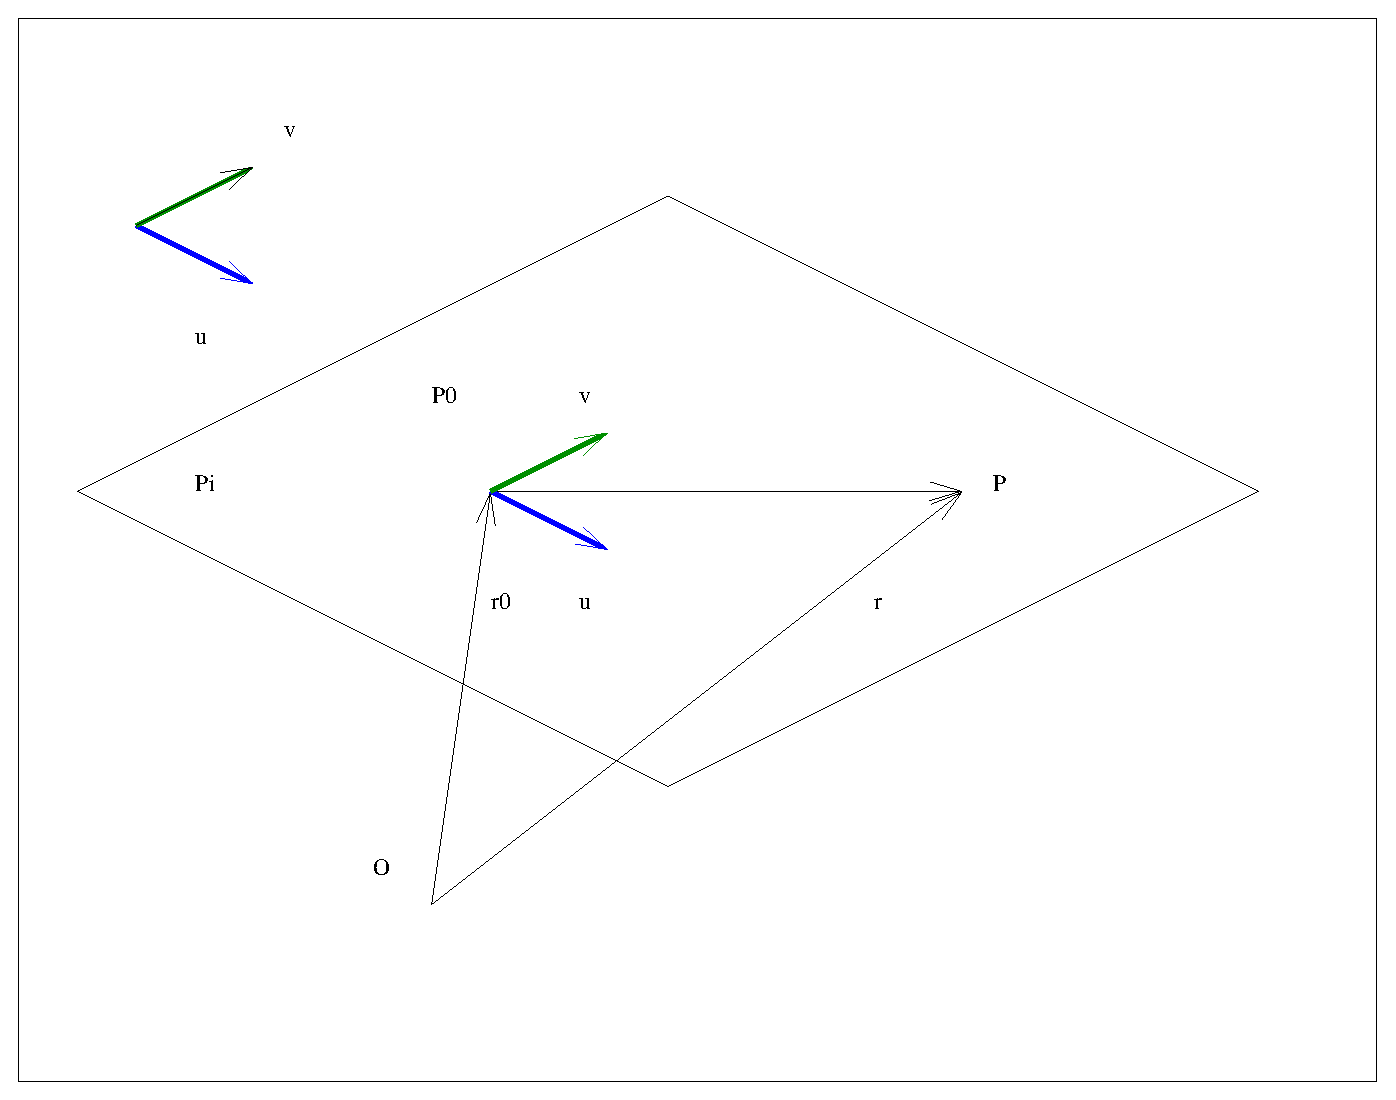
\includegraphics[height=2in]{../../modules/vectors/pictures/ok-plane_point_directions.eps}
    \end{figure}}
  \only<2>{\begin{figure}
        \psfrag{O}{$O$}
        \psfrag{Pi}{$\mathcal{P}$}
        \psfrag{P}{$P$}
        \psfrag{P0}{$P_0$}
        \psfrag{r}{$\textbf{r}$}
        \psfrag{n}{$\textbf{n}$}
        \psfrag{u}{$\textbf{u}$}
        \psfrag{v}{$\textbf{v}$}
        \psfrag{r0}{$\textbf{r}_0$}
        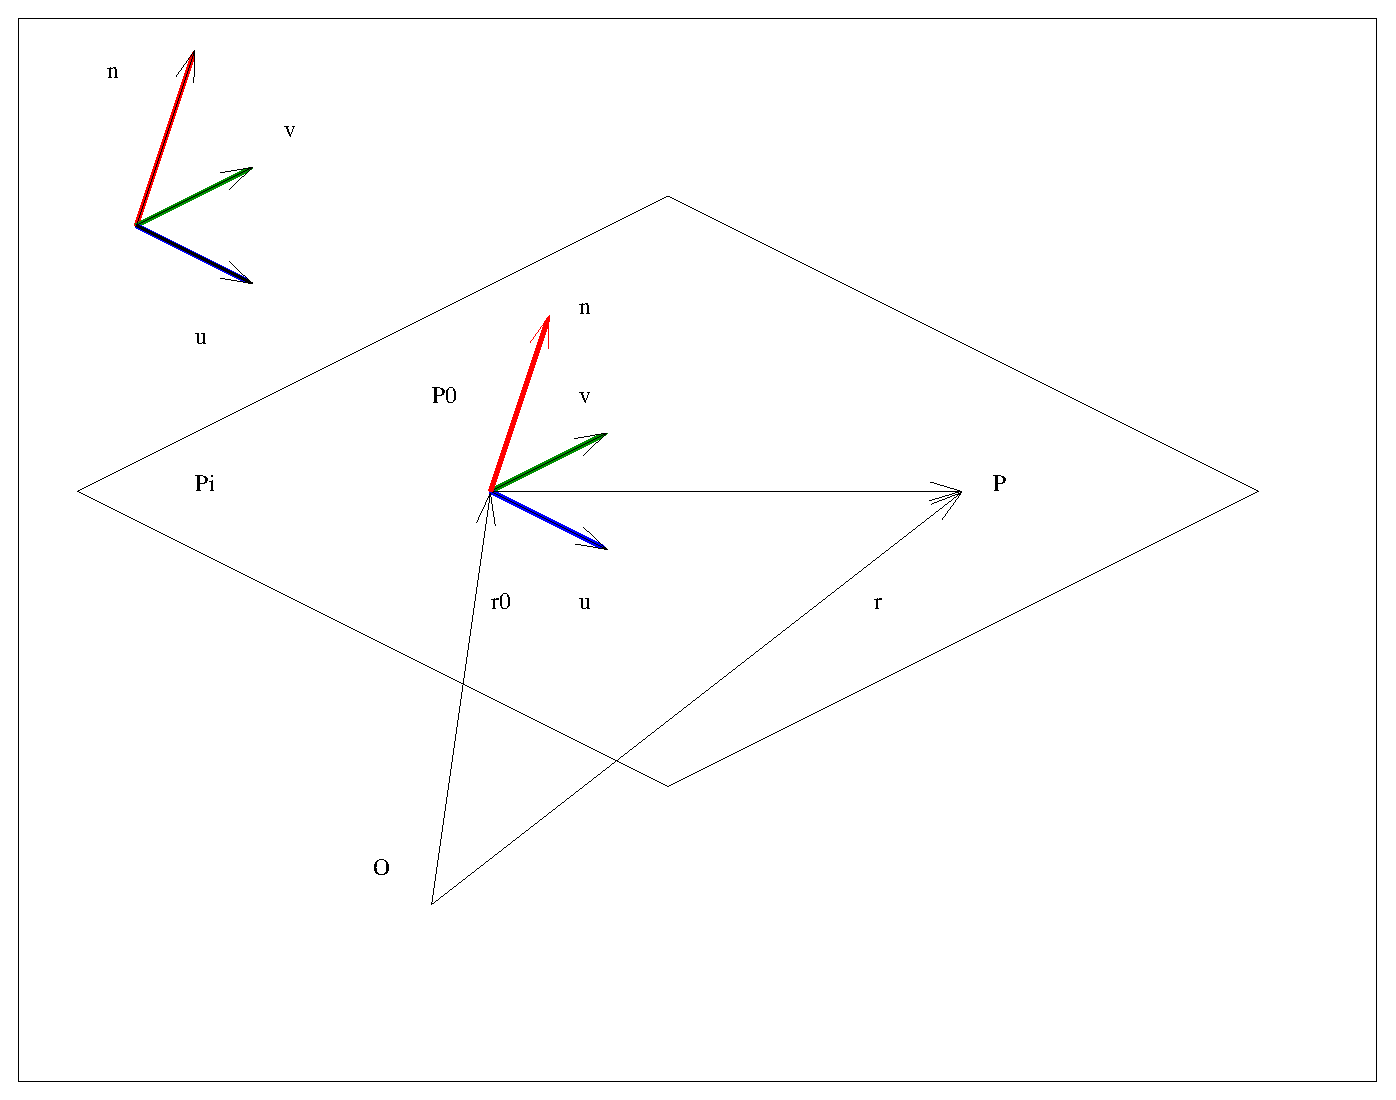
\includegraphics[height=2in]{../../modules/vectors/pictures/ok-plane_point_directions_vector.eps}
    \end{figure}}
    \only<3>{\begin{figure}
        \psfrag{O}{$O$}
        \psfrag{x}{$x$}
        \psfrag{y}{$y$}
        \psfrag{z}{$z$}
        \psfrag{Pi}{$\mathcal{P}$}
        \psfrag{P}{$P$}
        \psfrag{P0}{$P_0$}
        \psfrag{r}{$\textbf{r}$}
        \psfrag{n}{$\textbf{n}$}
        \psfrag{u}{$\textbf{u}$}
        \psfrag{v}{$\textbf{v}$}
        \psfrag{su}{$s\textbf{u}$}
        \psfrag{tv}{$t\textbf{v}$}
        \psfrag{r0}{$\textbf{r}_0$}
        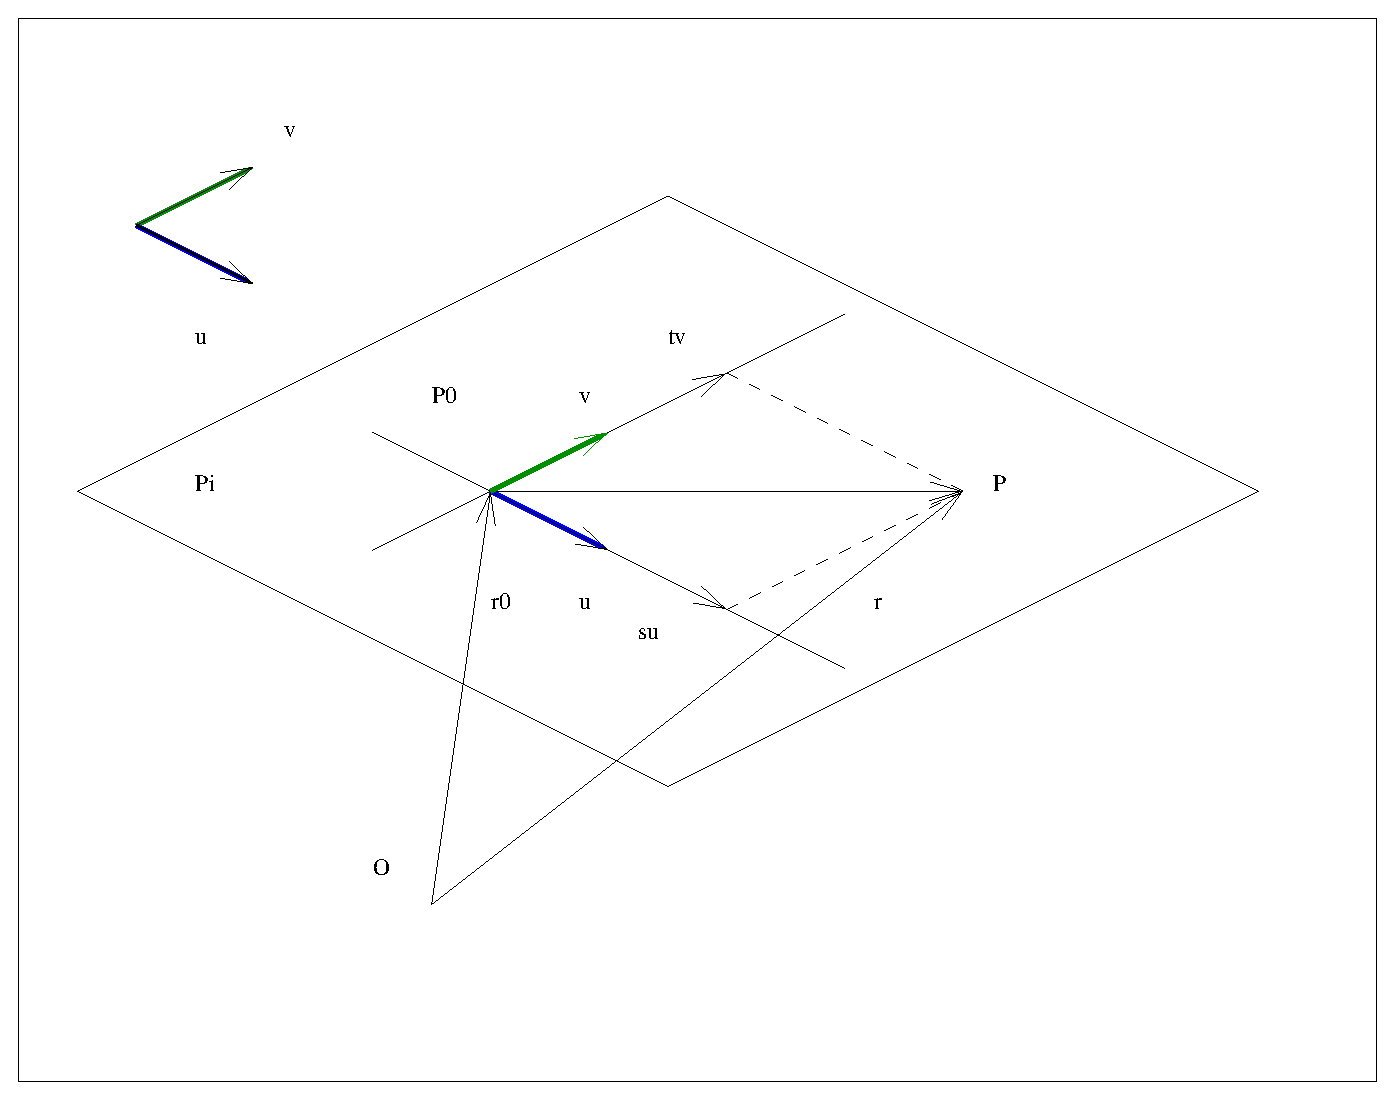
\includegraphics[height=2in]{../../modules/vectors/pictures/ok-plane_point_parametric_vectorial.eps}
    \end{figure}}
  \only<4>{\begin{figure}
        \psfrag{O}{$O$}
        \psfrag{x}{$x$}
        \psfrag{y}{$y$}
        \psfrag{z}{$z$}
        \psfrag{Pi}{$\mathcal{P}$}
        \psfrag{P}{$P$}
        \psfrag{P0}{$P_0$}
        \psfrag{r}{$\textbf{r}$}
        \psfrag{n}{$\textbf{n}$}
        \psfrag{u}{$\textbf{u}$}
        \psfrag{v}{$\textbf{v}$}
        \psfrag{su}{$s\textbf{u}$}
        \psfrag{tv}{$t\textbf{v}$}
        \psfrag{r0}{$\textbf{r}_0$}
        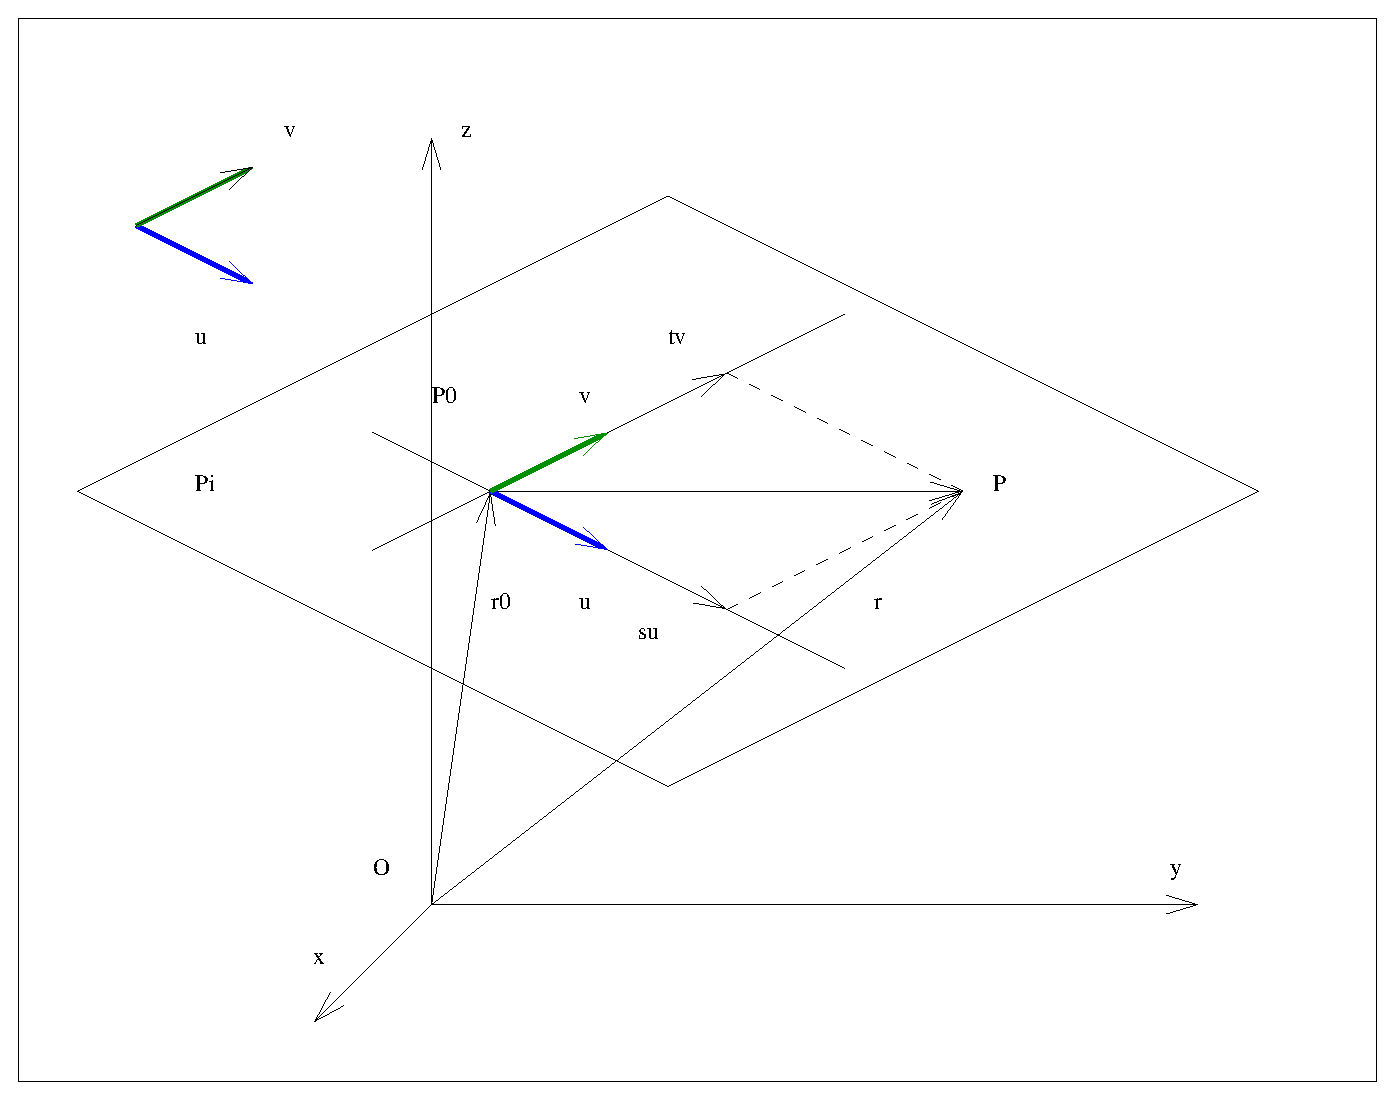
\includegraphics[height=2in]{../../modules/vectors/pictures/ok-plane_point_directions_scalar.eps}
    \end{figure}}
\end{columns}
\end{frame}


\begin{frame}
 \frametitle{Example}

$P_0(1,2,3)$, $\textbf{u}=\langle -1,0,2\rangle$, $\textbf{v} = \langle 0,-2,1\rangle$.\pause
%
$$\textbf{n} = \textbf{u} \times \textbf{v} = \left| \begin{array}{ccc}
                           \textbf{i} & \textbf{j} & \textbf{k} \\
			   -1 & 0 & 2 \\
                           0 & -2 & 1
                          \end{array}
\right| = 4\textbf{i}+\textbf{j} +2\textbf{k}$$
%
$$4(x-1)+1(y-2) + 2(z-3) = 0 \Longleftrightarrow 4x+y+2z = 12$$
%
\pause Implicit scalar equation:
%
$$4x+y+2z = 12\; .$$

\pause Parametric vectorial equation:
%
$$\langle x, y, z \rangle = \langle 1,2,3\rangle + s\langle -1, 0, 2\rangle + t\langle 0,-2,1\rangle$$

\pause Parametric scalar equations:
%
$$\left\{ \begin{array}{ll}
           x & = 1 -s \\
           y & = 2-2t \\
           z & = 3 +2s +t
          \end{array}
\right. \quad s,t \text{ real parameters}.$$
%
\end{frame}
